
% neue Folie
\newpage
\slidetitle{}
\section{Implementierung\\}
\begin{itemize}
	\item Repräsentation eines graphentheoretischen Baums\\
	
	\item L-System Implementierung\\
	
	\item Space Colonization Algorithmus Implementierung\\
	
	\item Modellgenerierungssystem
\end{itemize}






\newpage
\slidetitle{4. Implementierung - Baumrepräsentation}
\subsection{Baumrepräsentation\\}
\begin{itemize}
	
	\item Datenklasse zur Repräsentation eines graphentheoretischen Baums \\
	
	\item Objekte werden als Zylinder visualisiert\\
	
	\item Bietet Zugriff auf:
	\begin{itemize}
		\item Vorgänger und Nachfolger\\
		
		\item Modell-Daten\\
		
		\item Wachstums-Daten
	\end{itemize}
\end{itemize}





\newpage
\slidetitle{}
\subsection{Modellgenerierungssystem \\}
\begin{itemize}
	\item Eingabe eines graphentheoretischen Baums\\
	
	\item Vorbereitung der Modellgenerierung \\
	
	\item Generierung der Zylinder-Meshes\\
	
	\item Darstellung mithilfe des Grafiksystems
\end{itemize}





\newpage
\slidetitle{4. Implementierung - Modellgenerierungssystem}
\paragraph{Eingabe\\ }
\begin{itemize}
	\item Radius-Daten
	\item Genauigkeit \\
\end{itemize}
\paragraph{Vorbereitung\\ }
\begin{itemize}
	\item Kurvenreduktion
	\item Radiusberechnung
	\item Normalenberechnung
\end{itemize}





\newpage
\slidetitle{4. Implementierung - Modellgenerierungssystem}
\paragraph{Generierung der Zylinder-Meshes\\}


\begin{description}
	\item Grundlegende Idee: Verbindung zweier Kreise ergibt einen Zylindermantel
 
	\begin{itemize}
		\item Festlegung der Anzahl der Kreissegmente\\
		
		\item Berechnung der Vertizes auf den Kreisen\\
		
		\item Verbindung der Kreissegmente\\
		
		\item Generierung von Dreieck-Daten
	\end{itemize}
\end{description}




\newpage
\begin{center}
	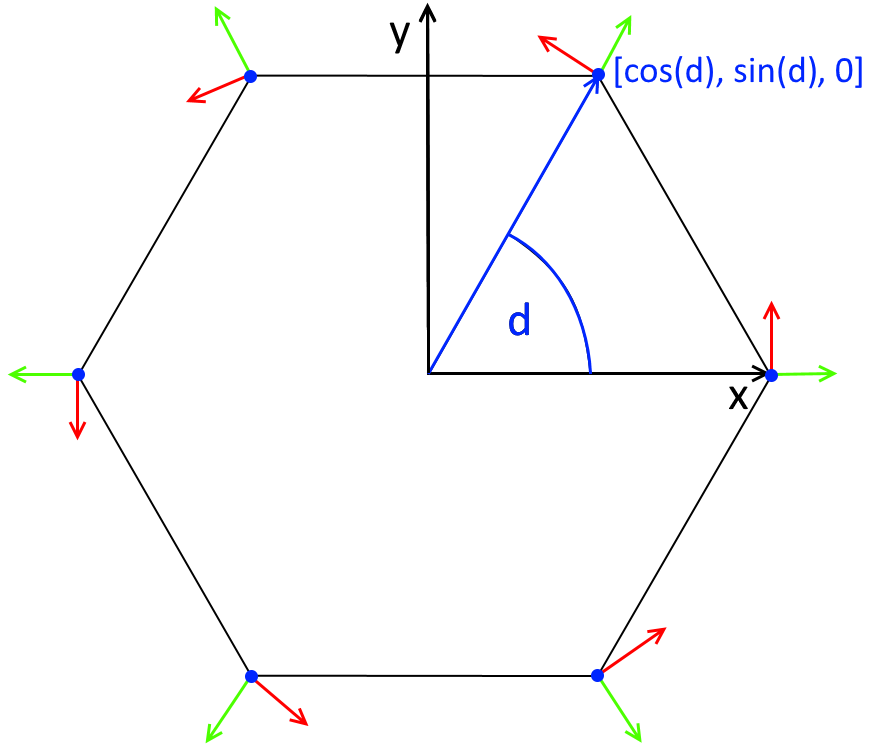
\includegraphics[height=.9\textheight]{images/CH4_Ring6Sections.png}
	
	Berechnung von Vertexposition auf einem Einheitskreis mit sechs Segmenten
\end{center}




\newpage
\begin{center}
	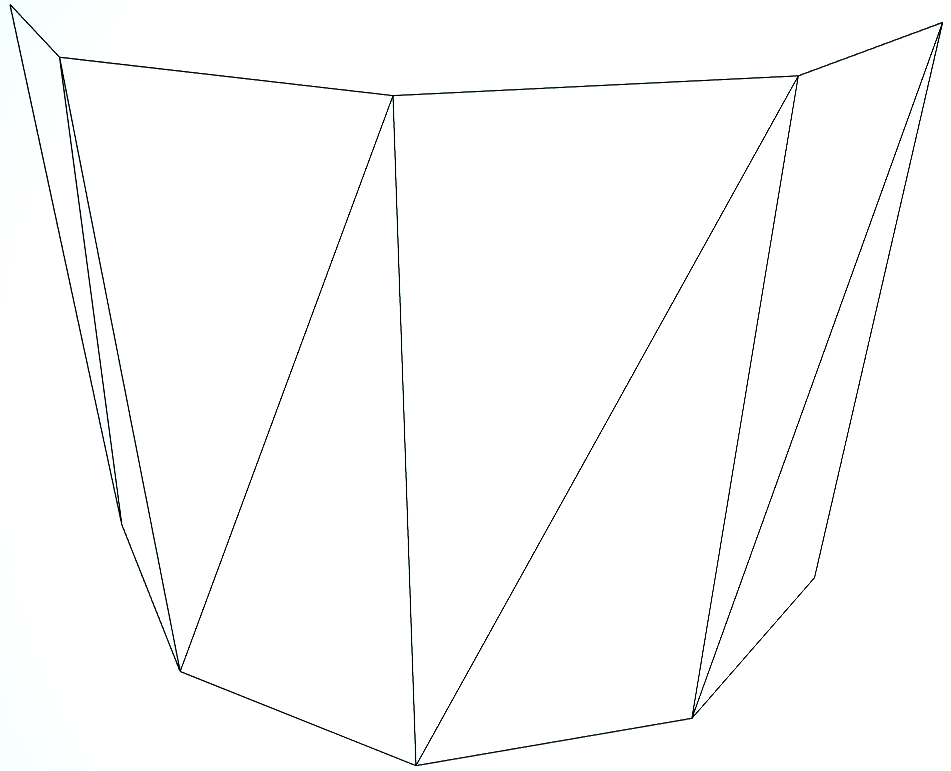
\includegraphics[height=.9\textheight]{images/CH4_Zylinder10SegmenteWireframe.png}
	
	Bei der Verbindung entstehende Dreiecke
\end{center}




\newpage
\begin{center}
	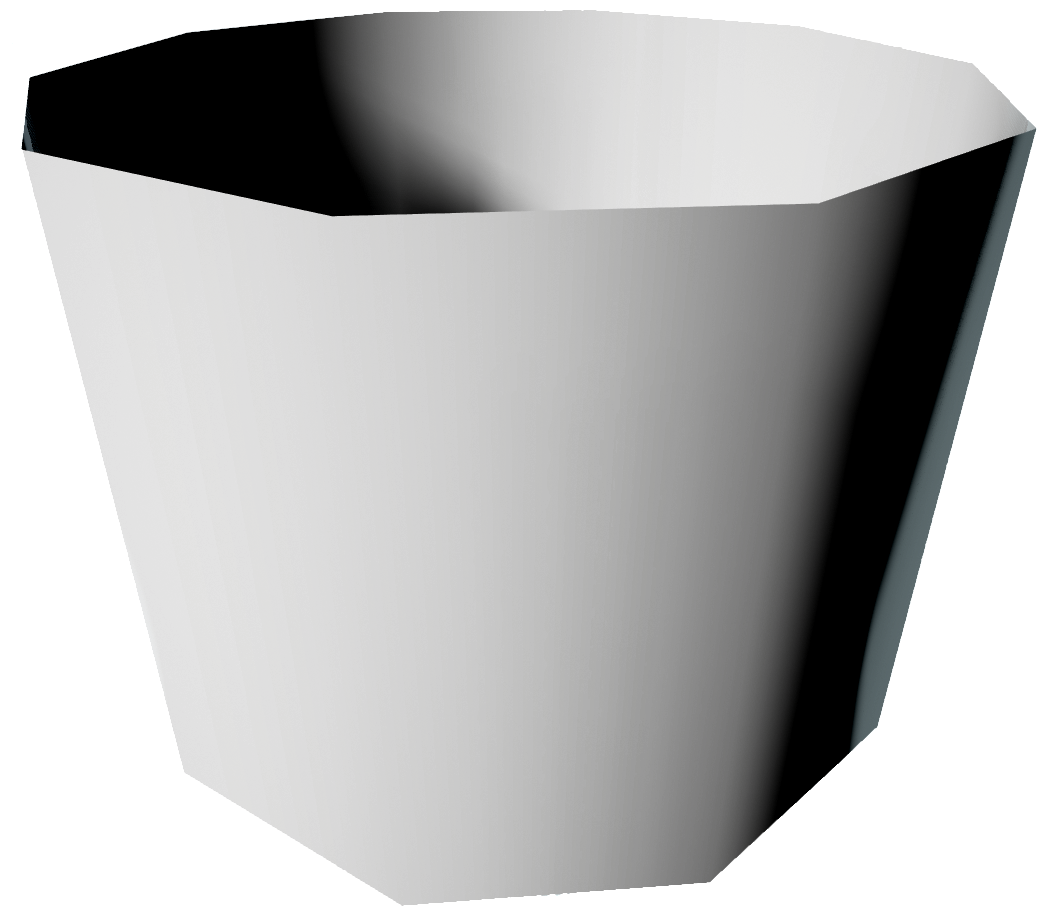
\includegraphics[height=.9\textheight]{images/CH4_Zylinder10SegmenteOpaque.png}
	
	Gefärbte Dreiecke mit Beleuchtung
\end{center}





